\documentclass[../main]{subfiles}

% Average J.du=du.j enjoyer

% feel free to edit this, just @ me if you make major changes

% to do: 
% - make results \ref'able
% - do commutative diagrams (done by George, thanks George)
% - use \varprojlim for limits

\begin{document}

\chapter{Duality in Manifolds}
\label{sec:p3c10}
In the classical case, to have a duality theorem relating $H_r(M;A)$ and $H^{m-r}(M;A)$ we need to assume $M$ is orientable, and then we can take $A$ to be any abelian group. Otherwise, we can suppose that $M$ is non-orientable; then either we must use twisted coefficients, or we must suppose that $A$ is a module over $\bbZ_2$. The point is that an orientable manifold has classes in $\bbZ$-homology and cohomology which enter into the statements and the proofs; and even a non-orientable manifold has such classes if we use homology and cohomology with coefficients in $\bbZ_2$. 

To generalise this situation, G.W. Whitehead introduced the notion of a \emph{ring-spectrum} and a \emph{module-spectrum}. The idea is that if $M$ is orientable with respect to $E_*$ and $E^*$, where $E$ is a ring-spectrum, then the duality theorem will hold for $F_*$ and $F^*$, where $F$ is any module-spectrum over $E$.
\begin{examples}
To illustrate the situation above, take
\[E=H, \ F=HA \ \text{ for any abelian group } A;\]
or
\[E = H\bbZ_2, \ F=HA \ \text{ for any $\bbZ_2$-module } A.\]
\end{examples}

A spectrum $E$ is said to be a \emph{ring-spectrum} \index{ring-spectrum} if it has given maps $\mu \colon E \wedge E \lra E$, $\eta \colon S \lra E$ of degree 0 such that the following diagrams commute.


\[
\begin{tikzcd}
E \wedge E \wedge E \arrow[dd, "1 \wedge \mu"'] \arrow[rr, "\mu \wedge 1"] &  & E \wedge E \arrow[dd, "\mu"] & S \wedge E \arrow[rr, "\eta \wedge 1"] \arrow[d] &  & E \wedge E \arrow[d, "\mu"] \\
                                                                           &  &                              & E \arrow[rr, "1"]                                &  & E                           \\
E \wedge E \arrow[rr, "\mu"]                                               &  & E                            & E \wedge S \arrow[rr, "1 \wedge \eta"] \arrow[u] &  & E \wedge E \arrow[u, "\mu"']
\end{tikzcd}
\]

Let $E$ is a ring-spectrum. We say a spectrum $F$ is a \emph{module-spectrum over $E$} \index{Module-spectrum} if it has given a map $\nu \colon E \wedge F \lra F$ of degree 0 such that the following diagrams commute.



\[
\begin{tikzcd}
E \wedge E \wedge F \arrow[dd, "1 \wedge \nu"'] \arrow[rr, "\mu \wedge 1"] &  & E \wedge F \arrow[dd, "\nu"] & S \wedge F \arrow[rr, "\eta \wedge 1"] \arrow[dd, "\cong"] &  & E \wedge F \arrow[dd, "\nu"] \\
                                                                           &  &                              &                                                   &  &                              \\
E \wedge F \arrow[rr, "\nu"]                                               &  & F                            & F \arrow[rr, "1"]                                 &  & F                           
\end{tikzcd}
\]


A ring-spectrum $E$ is said to be \emph{commutative} \index{commutative ring-spectrum} if the following diagram commutes.



\[
\begin{tikzcd}
E \wedge E \arrow[rr, "\mu"] \arrow[dd, "c"'] &  & E \\
                                              &  &   \\
E \wedge E \arrow[rruu, "\mu"']               &  &  
\end{tikzcd}
\]


If $E$ is a ring-spectrum, we can use the product map $\mu \colon E \wedge E \lra E$ to obtain products with values in $E_*$ or $E^*$ instead of $(E \wedge E)_*$ or $(E \wedge E)^*$. For example, we obtain a cup-product 
\[E^p(X,A) \otimes E^q(X,B) \lra E^{p+q}(X,A \cup B).\]
Similarly for an action map $\nu \colon E \wedge F \lra F$.

Practically all the examples of spectra which I have mentioned are, in fact, ring-spectra. I will only illustrate the case $E=H$. We have
\[\pi_r (H \wedge H) = H_r(H) = \begin{cases}
    0 & (r < 0) \\
    \bbZ & (r=0)
\end{cases}\]
so that by the Hurewicz theorem,
\[H_0(H \wedge H) = \bbZ.\]
Alternatively, by the Künneth theorem
\[H_0(H \wedge H) \cong H_0(H) \otimes H_0(H) \cong \bbZ \otimes \bbZ \cong \bbZ.\]
By the universal coefficient theorem,
\[H^0(H \wedge H) = \Hom(\bbZ,\bbZ) = \bbZ.\]
Therefore I can take a map $\nu \colon H \wedge H \lra H$ realizing the product map $\bbZ \otimes \bbZ \lra \bbZ$ of $\pi_0$.

Alternatively, realize $H \wedge H$ with no stable cells of dimension $d < 0$. Map the cells of dimension $0$ in the indicated way, and similarly for the cells of dimension $1$. Now the map extends over the higher stable cells of $H \wedge H$, because the higher homotopy groups of $H$ are zero. For the same reason, the map is unique up to homotopy.

For similar reasons, if $R$ is a ring then $HR$ is a ring-spectrum; if $M$ is an $R$-module then $HM$ is a module-spectrum over $HR$.

So far our generalised homology and cohomology theories have been defined on CW-pairs $X,A$. Now we would like to extend them to other categories of pairs.

We begin with the singular extension of $E_*$ and $E^*$. Take any pair $X,A$ and let $X',A'$ be a weakly equivalent CW-pair. Define the singular $E$-homology and $E$-cohomology groups of $X,A$ to be
\[E_p(X,A) = E_p(X',A'),\]
\[E^p(X,A) = E^p(X',A').\]
The result is independent of the choice of $X',A'$, up to a canonical isomorphism.

All the properties of $E_p$ and $E^p$ carry over very well, except for excision. Here one has to be careful. Let $U \cup V$ be a space which comes as the union of two subspaces $U$ and $V$ intersecting in $U \cap V$. Then we can certainly take a CW-complex $W'$ equipped with a weak equivalence
\[W' \lar{w}U \cap V,\]
and we can enlarge $W'$ on the one hand to a CW-complex $U'$ admitting a weak equivalence 
\[U' \lar{u} U\]
extending $w$, and on the other hand to a CW-complex $V'$ admitting a weak equivalence 
\[V' \lar{v} V\]
also extending $w$. Then we can put them together to get
\[U' \cup_{W'} V' \lra  U \cup V.\]
But this map is not a weak equivalence in general. For example, take subsets of the real numbers; let $U = \bbQ$, $V=\bbR - \bbQ$; then $W'$ will be empty, $U'$ will be a countable discrete space, and $U' \cup_{W'} V'$ will be an uncountable discrete space, which is not weakly equivalent to $\bbR$.

However, if we assume that $\Int U \cup \Int V = U \cup V$, then $U' \cup_{W'} V' \lra U \cup V$ is a weak equivalence, and all is well. So the excision axiom holds with this extra hypothesis, which is actually the standard one for ordinary (singular) homology and cohomology.

I must also comment on the behaviour of singular homology for limits. Let $X,Y$ be a pair containing a directed family of subpairs $X_\alpha,Y_\alpha$. Then we can form
\[\varinjlim_\alpha E_p(X_\alpha,Y_\alpha) \lra E_p(X,Y).\]
\begin{proposition}\label{prop:p3c10.1}
In order that this map be an isomorphism, it is sufficient that for any compact pair $K,L \subset X,Y$ we can find an $\alpha$ such that $X_\alpha,Y_\alpha \supset K,L$.
\end{proposition}

The proof is easy.

Now I want to define a \v{C}ech-type cohomology theory \index{\v{C}ech-type cohomology theory} for compact pairs $K,L$ which happen to come embedded in some topological manifold $M$, possibly not compact, possibly with boundary. The definition is as follows. Let $U,V$ run over open pairs in $M$ with $U \supset K, V \supset L$. These form a directed set; if $U_i \supset K$, $V_i \supset L$ for $i=1,2$ then $U_1 \cap U_2 \supset K$, $V_1 \cap V_2 \supset L$. So I define
\[\check{E}^*(K,L) = \varinjlim_{(U,V)} E^*(U,V).\]
(The notation $E^*$, when applied to an arbitrary topological pair $X,A$ will mean singular $E$-cohomology). Of course we will always have a map 
\[E^*(U,V) \lra E^*(K,L);\]
this passes to the limit, and gives us a map
\[\check{E}^*(K,L) \lra E^*(K,L).\]
In general this map need not be an isomorphism. However, there are cases when it is.
\begin{examples}[i]
Suppose that $M$ is a compact topological manifold, possibly with boundary. Then 
\[\check{E}^*(M) \lra E^*(M)\]
is an isomorphism.
\end{examples}
In fact, the pair $M,\emptyset$ qualifies as an open pair containing the compact pair $M,\emptyset$, and is terminal.
\begin{examples}[ii]
Suppose $K$ is a point $x$. Then 
\[\check{E}^*(x) \lra E^*(x)\]
is an isomorphism.
\end{examples}

In fact, any point $x$ lies in a coordinate neighbourhood, so we can choose a cofinal system of open pairs $U_\alpha, \emptyset \supset x, \emptyset$ with $U_\alpha$ contractible. Then 
\[E^*(U_\alpha) \lra E^*(x)\]
is an isomorphism for all $\alpha$.

Next I would like to know that $\check{E}^*(K,L)$ is a topological invariant of the pair $(K,L)$, and does not depend on the embedding in $M$.
\begin{lemma}[i]\label{lem:p3c10.2}

Suppose given compact pairs $K_1,L_1 \subset M_1$ and $K_2,L_2 \subset U_2,V_2 \subset M_2$, where $U_2,V_2$ is an open pair, and a continuous map
\[f \colon K_1,L_1 \lra K_2,L_2.\]
Then $f$ can be extended so as to map some open pair $U_1,V_1 \supset K_1,L_1$ in $M_1$ to $U_2,V_2$.

(ii) Suppose given a homotopy 
\[h \colon I \times K_1,I \times L_1 \lra K_2,L_2,\]
and extensions $f^0$ of $h^0$, $f^1$ of $h^1$ which map (possibly different) open pairs $U^0,V^0$ and $U^1,V^1$ into an open pair $U_2,V_2 \supset K_2,L_2$. Then there exists an open pair pair $U,V$ with $K_1,L_1 \subset U,V \subset U^0 \cap U^1,V^0 \cap V^1$ and a homotopy 
\[h \colon I \times U, I \times V \lra U_2,V_2\]
extending $f^0|_{U,V}$, $f^1|_{U,V}$ and $h$.
\end{lemma}
\begin{proof}
Standard but repeated use of compactness, plus the Tietze extension theorem; we rely heavily on the fact that $M_2$ is a manifold.
\end{proof}
\begin{corollary}\label{cor:p3c10.3}
A map $f \colon K_1 , L_1 \lra K_2,L_2$ induces $f^* \colon \check{E}^*(K_2,L_2) \lra \check{E}^*(K_1,L_1)$ depending only on the homotopy class of $f$, and satisfying $1^* = 1$, $(fg)^* = g^* f^*$.
\end{corollary}

The exactness properties of $\check{E}^*$ are fine, since direct limits preserve exactness.

\begin{examples}
Let $M, \partial M$ be a pair consisting of a compact topological manifold with boundary and its boundary. Then 
\[\check{E}^*(M,\partial M) \lra E^*(M,\partial M)\]
is an isomorphism.
\end{examples}
\begin{proof}
Consider the following commutative diagram.

\[
\begin{tikzcd}[column sep = 2em]
\dots \arrow[r] & {\check{E}^\ast(M,\partial M)} \arrow[r] \arrow[dd] & \check{E}^\ast(M) \arrow[dd, "\cong"] \arrow[r] & \check{E}^\ast(\partial M) \arrow[dd, "\cong"] \arrow[r, "\delta"] & {E^\ast(M,\partial M)} \arrow[dd] \arrow[r] & \dots \\
                &                                                     &                                                 &                                                                    &                                             &       \\
\dots \arrow[r] & {E^\ast(M,\partial M)} \arrow[r]                    & E^\ast(M) \arrow[r]                             & E^\ast(\partial M) \arrow[r, "\delta"]                             & {E^\ast(M,\partial M)} \arrow[r]            & \dots
\end{tikzcd}
\]
The rows are exact, and the two arrows marked are isomorphisms by a previous example. The result follows by the 5-lemma.
\end{proof}

N.B. This way of saying things relies on the previous proof that $\check{E}^*(\partial M)$ is independent of the embedding of $\partial M$ in $M$, but it does not need the construction of a collar for $\partial M$ inside $M$.

The excision properties of $\check{E}^*$ are excellent, because $\check{E}^*$ was defined using only open pairs in $M$.
\begin{proposition}\label{prop:p3c10.4}
If $U,V$ are any compact sets in $M$, then
\[\check{E}^*(U \cup V,V) \lra \check{E}^*(U,U \cap V)\]
is an isomorphism.
\end{proposition}

This follows from the definitions by a bit of general topology (compact Hausdorff spaces again.)

I also have to comment on the behaviour of $\check{E}^*$ for limits.
\begin{proposition}\label{prop:p3c10.5}
Let $K_\alpha,L_\alpha$ be a downward-directed set of compact pairs in $M$, with intersection $K,L$. Then 
\[\varinjlim_{\alpha} \check{E}^*(K_\alpha,L_\alpha) \lra \check{E}^*(K,L)\]
is an isomorphism.
\end{proposition}
Again, this is easy modulo a bit of general topology. One must show that given any open pair $U,V \supset K,L$ there is an $\alpha$ with $K_\alpha,L_\alpha \subset U,V$.

Experience in Manchester and Cambridge suggests I had better give some exposition about orientations. Suppose $E\lar{p} B$ is an $n$-plane bundle and $E^0$ is the complement of the zero cross-section. Then for each point $x \in B$, I have the fibre $E_x = p^{-1}x$; let $E^0_x= E_x \cap E^0$. I can form
\[H_n(E_x,E_x^0) \cong \bbZ \]
\[H^n(E_x, E_x^0) \cong \bbZ.\]
Now since $E \lar{p} B$ is a bundle, locally it is a product; and if $x$ and $y$ are close together we can easily tell which element in $H_n(E_x,E_x^0)$ corresponds to which in $H_n(E_y,E_y^0)$. That is, we get a bundle over $B$, with fibre $\bbZ$, and with structure group $\bbZ_2$ acting on $\bbZ$ by $n \mapsto -n$. A similar situation occurs in cohomology.

One may say that the original $n$-plane bundle was \emph{orientable} if the $\bbZ$-bundle $\bigcup_x H_n(E_x,E_x^0)$ is trivial. The definition may be given equally well in terms of homology or cohomology; we have
\[H^n(E_x,E_x^0) = \Hom(H_n(E_x,E_x^0),\bbZ),\]
so the two bundles are trivial or non-trivial together.

If we are given orientations consistently on each fibre, that amounts to saying there is a continuous section
\[\lambda \colon B \lra \bigcup_x H_n(E_x,E_x^0)\]
which assigns to each point $x \in B$ a generator 
\[\lambda(x) \in H_n(E_x,E_x^0) \cong \bbZ.\]
The same goes to cohomology. But I would like a statement more global than that. In this case it is clear that cohomology rather than homology is required. Suppose, for example, that $B$ had an infinity of path-components; then a singular homology class could only have a non-zero component in a finite number of them, but this difficulty does not arise in cohomology. We can ask if there is an element 
\[\omega \in H^n(E,E^0)\]
such that for each $x \in B$, the induced homomorphism 
\[i_x^* \colon H^n(E,E^0) \lra H^n(E_x,E_x^0)\]
has $i_x^* \omega = \lambda(x)$ for any given section $\lambda$.

Now in ordinary homology, the answer is yes: if you are given a section $\lambda$, there exists a cohomology class $\omega$ such that $i_x^* = \lambda(x)$ for each $x$, and $\omega$ is unique. However, the proof makes essential use of the dimension axiom. For a generalised cohomology theory the corresponding result is not true. There is an $n$-plane bundle $E \lra B$ and a section $\lambda \colon B \lra \bigcup_x \te{KO}^n(E_x,E_x^0)$ such that there exists no $w \in \te{KO}^n(E,E^0)$ with $i_x^* \omega = \lambda(x)$ for all $x$; in another such example the required $\omega$ exists but is not unique.

It seems best to choose our definitions so as to avoid the difficulty. First I consider the meaning to be assigned to the word ``generator.'' Let $F$ be a ring-spectrum; then $F_*(\bbR^n,\bbR^n-0) = \tilde{F}_*(S^n)$ and $F^*(\bbR^n,\bbR^n-0) = \tilde{F}^*(S^n)$ are modules over $\pi_*(F)$. In fact each is a free module on one generator, because we have canonical classes
% Note that the second item here only reads $\gamma^n \in F^n(\bbR^n - 0)$ in the original text, but that's obviously nonsense and I'm (very nearly) certain that this here is what's intended
\[
	\gamma_n \in F_n(\bbR^n,\bbR^n-0), \quad \gamma^n \in F^n(\bbR^n, \bbR^n - 0).
\]
I will say that $\varphi \in F^*(\bbR^n,\bbR^n-0)$ is a \emph{generator} \index{generator of ring-spectrum} if $\{\varphi\}$ is a $\pi_*(F)$-base for $F^*(\bbR^n,\bbR^n-0)$. $\varphi$ is a generator if and only if $\varphi = u \gamma^n$, where $u$ is a unit in $\pi_*(F)$. $\varphi$ need not lie in $F^n(\bbR^n,\bbR^n-0)$, because we may have units of non-zero degree in $\pi_*(F)$; e.g., this occurs if $F=K$.

The property which I need of generators is the following. Let $G$ be a module-spectrum over $F$. Then the map \[G_*(\bbR^n,\bbR^n-0) \lra \pi_*(G)\]
given by 
\[y \mapsto  \langle \varphi , y \rangle\]
is an isomorphism. In fact it is trivially so if $\varphi = \gamma^n$, and the general case differs only by a unit in $\pi_*(F)$.

We say $\omega \in  F^*(E,E^0)$ is an \emph{orientation} \index{orientation} for $E$ if
\[i_x^* \omega \in F^*(E_x,E_x^0)\]
is a generator for each $x \in B$.

Of course, the question of constructing an orientation for a vector-bundle, or of constructing orientations for some class of bundles, is non-trivial. However it can be done in several cases which are important in the applications. For example, complex $n$-plane bundles can be oriented over $K^*$ or $\te{MU}^*$; Spin bundles can be oriented over $\te{KO}^*$; and so on. I will not give the constructions here.

We have defined orientations as they apply to $n$-plane bundles; but we want the notion as well for topological manifolds, which might not have a tangent bundle in the same sense as smooth manifolds. But it is well known what one substitutes for the tangent bundle. That is, one replaces $E$ by $M \times M$, where $M$ is a topological manifold, say without boundary. One replaces $E^0$ by the complement of the diagonal, $M \times M - \Delta$. One replaces the fibres $E_x$ by the fibres $x \times M$ of the projection $p_1 \colon M \times M \lra M$. One replaces $E^0_x$ by $x \times M - x \times x$. Since $M$ is a topological manifold without boundary, $x$ has a neighbourhood $U$ in $M$ which is homeomorphic to a neighbourhood of 0 in $\bbR^n$, by a homeomorphism mapping $x$ onto 0. Then $F^*(M,M-x) \cong F^*(U,U-x)$ by excision and so is isomorphic to $F^*(\bbR^n,\bbR^n - 0)$.

By an \emph{orientation}\index{Orientation for tangent bundle} over $F^*$ for the tangent bundle of a topological manifold $M$, we will therefore mean a class $\omega \in F^*(M \times M, M \times M - \Delta)$ such that
\[i_x^* \omega \in F^*(x \times M, x \times M - x \times x)\]
is a generator for each $x$. 

If $M$ happens to have a boundary, there are two things we can do. The first starts from the observation that for a smooth manifold $M$, the tangent bundle to $M$ contains over $\partial M$ tangent vectors which point out, as well as tangent vectors which point in. To copy this in the topological case, one adds an open collar on the boundary; that is, one forms
\[M' = M \cup [0,1) \times \partial M.\]
This is a topological manifold without boundary, and it has a fully satisfactory topological tangent bundle, and one can ask for an orientation.

The other thing we can do is to use the same form of words as before, and ask for a class
\[F^*(M \times M, M \times M - \Delta)\]
but only demand that $i_x^* \omega$ be a generator for $x \in M - \partial M$.

Evidently the first sort of orientation restricts to the second, but I will not go into the relations between them.

Having completed the discussion of bundles, we go back to using $E$ for a ring-spectrum.

Suppose given an orientation class
\[\omega \in E^d(M \times M, M \times M - \Delta),\]
where $E$ is a ring-spectrum. Let $F$ be the module-spectrum over $E$. We define a duality map, which ultimately will be a map of the following form. Let $K,L$ be a compact pair in $M$. Then $M-L,M-K$ is an open pair in $M$. The duality map will be a homomorphism
\[D \colon F_p(M-L,M-K) \lra \check{F}^{d-p}(K,L)\]
where the left-hand side, as before, indicates singular $F$-homology.

We will define the map $D$ in a number of steps. Let $U,V \supset K,L$ be an open pair and $V',U'$ another open pair with $U \cap U' = \emptyset$, $V \cap V' = \emptyset$. Then we have
\[U \times U' \subset M \times M - \Delta\] 
\[V \times V' \subset M \times M - \Delta.\]
Therefore we can form
\[i^* \omega \in E^d(U \times V', U \times U' \cup V \times V').\]
So given $x \in F_p(V',U')$ we can form
\[D(x) = (i^* \omega)/x \in F^{d-p}(U,V).\]

I claim $D$ is natural for inclusion maps. First, suppose $U'' \subset U$, $V'' \subset V$. Then surely $U'' \cap U' = \emptyset$, $V'' \cap V' = \emptyset$. The following diagram commutes.


\[
\begin{tikzcd}
                          & {F_p(V',U'')} \arrow[ldd] \arrow[rdd] &                    \\
                          &                                       &                    \\
{F^{d-p}(U,V)} \arrow[rr] &                                       & {F^{d-p}(U'',V'')}
\end{tikzcd}
\]


Next suppose $V''',U''' \subset V',U'$. Again $U''' \cap U' = \emptyset$, $V''' \cap V = \emptyset$. The following diagram commutes.
\[
\begin{tikzcd}
{F_p(V''', U''')} \arrow[rd] \arrow[rr] &                   & {F_p(V', U')} \arrow[ld] \\
                                        & {F^{d - p}(U, V)} &                         
\end{tikzcd}
\]
Both facts are immediate from \ref{prop:p3ch09.1}.

Again, I claim that $D$ commutes with boundary maps, up to a suitable sign. More precisely, suppose we have
\[U \supset V \supset W \qquad U' \subset V' \subset W'\]
with $U \cap U' = \emptyset$, $V \cap V' = \emptyset$, $W \cap W' = \emptyset$. Then the diagram
\[
\begin{tikzcd}
{F_p(W', V')} \arrow[rr, "\partial"] \arrow[dd, "D"] &              & {F_{p - 1}(V', U')} \arrow[dd, "D"] \\
                                                     & (-1)^{d + 1} &                                     \\
{F^{d - p}(V, W)} \arrow[rr, "\delta"]               &              & {F^{d - p + 1}(U, V)}              
\end{tikzcd}
\]
commutes up to the sign $(-1)^{d+1}$. For we can easily reduce it to the case $W = \emptyset, U' = \emptyset$, by the following diagram.
\[
\begin{tikzcd}[column sep = {5.8em, between origins}]
                             & {F_p(W', V')} \arrow[ld] \arrow[rd]\arrow[rr, "\partial"] &                                                & {F_{p - 1}(V', \emptyset)} \arrow[rd] \arrow[rr] &                       & {F_{p - 1}(V', U')} \arrow[ld] \\
{F^{d - p}(V, W)} \arrow[rr] &                                                 & {F^{d - p}(V, \emptyset)} \arrow[rr, "\delta"] &                                                  & {F^{d - p + 1}(U, V)} &                               
\end{tikzcd}
\]

Now since $\omega \in E^d(U \times W',V \times V')$ and by \ref{thm:p3ch09.12}(ii) we have
\[
	\delta((i^* \omega)/x) = (-1)^{d+1}(j^* \omega)/\partial x.
\]

Now we can start to pass to limits. Let us take a compact pair $K,L \subset M$ and consider the complementary open pair $M-L,M-K$. We vary $V',U'$ over open pairs contained in $M-L,M-K$, of course arranging that $U \cap U' = \emptyset$, $V \cap V' = \emptyset$. Now $\check{F}^*(K,L) = \varinjlim F^*(U,V)$, so with a class in $\check{F}^*(U,V)$ for any $U,V$ we get an image in $\check{F}^*(K,L)$. Now I claim that for any $x \in F_p(V',U')$, its image in $\check{F}^{d-p}(K,L)$ is independent of the choice of pair $U,V$, provided, of course, that there exists a pair $U,V \supset K,L$ with $U \cap U' = \emptyset$, $V \cap V' = \emptyset$. And this is immediate, by the following diagram.
\[
\begin{tikzcd}
                             & {F_p(V', U')} \arrow[dd] \arrow[rd] \arrow[ld] &                                  \\
{F_{d - p}(U, V)} \arrow[rd] &                                                & {F_{d - p}(U'', V'')} \arrow[ld] \\
                             & {F_{d - p}(U \cap U'', V \cap V'')}            &                                 
\end{tikzcd}
\]
So now we have a well-defined function 
\[D \colon F_p(V',U') \lra \check{F}^{d-p}(K,L).\]
(In fact, if $V''',U''' \subset V',U'$ and there exists a pair $U,V$ with $U \cap U' = \emptyset, V \cap V' = \emptyset$, then the following diagram commutes.)
\[
\begin{tikzcd}
{F_p(V''', U''')} \arrow[rr] \arrow[rd] &                   & {F_p(V', U')} \arrow[ld] \\
                                        & {F^{d - p}(U, V)} &                         
\end{tikzcd}
\]
But I claim we have
\[\varinjlim_{(V',U')} F_p(V',U') \lra F_p(M-L,M-K).\]
For this we need only check, by general topology, that the available pairs $(V',U')$ satisfy \ref{rmk:p3c10.10}.

At this stage, then, we have a transformation
\[D \colon F_p(M-L,M-K) \lra \check{F}^{d-p}(K,L)\]
which is natural in the sense that it commutes with the homomorphisms induced by inclusion maps, and, up to a sign $(-1)^{d+1}$, with the boundary maps.
\begin{theorem}\label{thm:p3c10.6}
$D$ is an isomorphism if $K \cap \partial M \subset L$.
\end{theorem}
We build up the proof by stages. We always assume our pairs $K,L$ have $K \cap \partial M \subset L$.
\begin{remark}\label{rmk:p3c10.7}
$D$ is an isomorphism if $K$ is a point $x$, and $L = \emptyset$.
\end{remark}
\begin{proof}
Our assumption is $x \cap \partial M \subset L = \emptyset$, so $x \not\in \partial M$. I claim the following diagram is commutative.
\[
\begin{tikzcd}
{F_p(M, M - x)} \arrow[rrd, "g"'] \arrow[rr, "D"] &  & \breve F^{d - p}(x) \arrow[d, "\cong"] \\
                                                  &  & F^{d - p}(x)                          
\end{tikzcd}
\]
Here $g(y) = \langle i_x^* \omega, y \rangle$. Our assumption is that $i_x^* \omega$ is a generator, so the Kronecker product with it is an isomorphism.

The commutativity of the diagram follows easily from naturality. We can begin by supposing that we start from a class in $F_p(M,M-x)$ which comes from $y \in F_p(M,M-B)$, where $B$ is a small closed ball in a coordinate neighbourhood. (This uses \ref{prop:p3c10.1}.) If we apply $D$ and the map into $F^{d-p}(x)$, we obtain
\[j^*((i^* \omega)/y),\]
where $j \colon x \lra \Int B$ is the injection. We have
\[
	j^*((i^*\omega/y) = ((j \times 1)^* i^* \omega)/y = i_x^*\omega/y = \langle i_x^* \omega, y \rangle. \qedhere
\]
\end{proof}
\begin{remark}\label{rmk:p3c10.8}
Suppose $K$ is a rectilinear simplex in a coordinate neighborhood and $L$ is one face of $K$ (which may be $K$ but must not be $\emptyset$). Then $D$ is an isomorphism between groups which are zero.
\end{remark}
Note: coordinate neighborhoods are supposed to map $\partial M$ into a linear subspace of $\bbR^n$, e.g., $\bbR^{n-1}$.
\begin{proof}
(i) $\check{F}^*(K,L) = 0$. In fact, we can even show this without appealing to the homotopy invariance of $\check{F}^*$; just surround $K,L$ by a confinal system of open convex neighborhoods $U,V$, for which $F^*(U,V) = 0$.

(ii) Also $F_*(M-L,M-K) = 0$. This is seen geometrically; see the accompanying figure. We can write $K$ as the join $K = L * K'$. If $K' = \emptyset$, $K = L$ then the result is trivially true.  Since $K' \cap \partial M = \emptyset$, we can draw a slightly larger simplex $K''$ slightly farther away from $L$ so that $L*K''$ is $n$-dimensional and contains $L * K'$, while $L*K' \cap \partial(L*K'') = L$. Then $(L*K'')-L$ is homeomorphic to $L \times (0,1] \times K'' \cup K''$:
% TODO layout. there's a big, ugly void caused by this here
\[
\begin{tikzpicture}[scale = .9]
    \draw (0, 2) to (0, 0) to (5, 0) to (5, 2);
    \draw[dashed] (5, 2) to (4, 2);
    \draw (4, 2) to (4, 1.25) to (1, 1.25) to (1, 2);
    \draw[dashed] (1, 2) to (0, 2);
\end{tikzpicture}\qquad
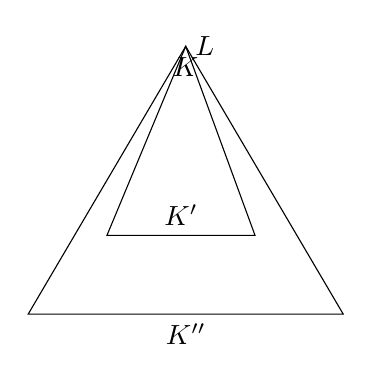
\begin{tikzpicture}[scale = .8]
    \draw (0, 0) to node[below] {$K''$} (5, 0) to (2.5, 4.25) node[right] {$L$} to cycle;
    
    \draw (2.5, 4.25) node[below=0.5] {$K$} to (1.25, 1.25) to node[above] {$K'$} (3.6, 1.25) to cycle;
\end{tikzpicture}
\]
Now clearly $L*K'' - L*K' \lra L*K'' - L$ is a homotopy equivalence, by maps and homotopies keeping $\partial(L* K'') - L$ fixed throughout. These maps and homotopies extend over $M$ by keeping everything fixed outside $L*K''$. 
\end{proof}
\begin{remark}\label{rmk:p3c10.9}
Suppose $K$ is a rectilinear simplex in a coordinate neighborhood and $L = \emptyset$. Then $D$ is an isomorphism.
\end{remark}
\begin{proof}
Since $L = \emptyset$, we have $K \cap \partial M = \emptyset$. Let $x$ be one vertex of $K$. Then we have the following commutative diagram.
\[
\begin{tikzcd}[column sep = tiny, font = \footnotesize]
0 = {F_p(M -x, M - K)} \arrow[r]       & {F_p(M, M- K)} \arrow[d] \arrow[r] & {F_p(M, M - x)} \arrow[d, "\cong"] \arrow[r] & {F_{p - 1}(M - x, M - K)} = 0 \\
0 = {\breve F^{d - p}(K, x)} \arrow[r] & \breve F^{d - p}(K) \arrow[r]      & \breve F^{d - p}(x) \arrow[r]                & {\breve F^{d - p + 1}(K, x)} = 0
\end{tikzcd}
\]
The four groups marked zero are so by \ref{rmk:p3c10.8}. The map marked as an isomorphism is so by \ref{rmk:p3c10.7}.
\end{proof}
\begin{remark}\label{rmk:p3c10.10}
Suppose $K_1,L_1$ and $K_2,L_2$ are compact pairs in $M$ with $K_1 \cap \partial M \subset L_1$, $K_2 \cap \partial M \subset L_2$, and $K_1 \cap L_2 = L_1 \cap K_2$. If $D$ is an isomorphism for $(K_1,L_1)$, $(K_2,L_2)$ and $(K_1\cap K_2,L_1 \cap L_2)$, then it is an isomorphism for $(K_1 \cup K_2, L_1 \cup L_2)$.
\end{remark}
\begin{proof}
Consider the diagram of Mayer-Vietoris sequences on the following page. The Mayer-Vietoris sequences are slightly more general than those considered in Eilenberg and Steenrod but none the worse for that. The second row works because $K_1 \cap L_2 = L_1 \cap K_2$; this is the condition that the Mayer-Vietoris sequence may be replaced by one in which the subspaces remain fixed (namely at $L_1 \cup L_2$). The first row works for the dual reason that
\[(M-K_1) \cup (M-L_2) = (M-L_1) \cup (M-K_2);\]
this is the condition that the Mayer-Vietoris sequence may be replaced by one in which the subapces remain fixed (namely at $(M-L_1) \cup (M-L_2)$) and the subspaces vary. We have the excision necessary for the first row because all the subspaces are open, and for the second because excision always holds for \v{C}ech $F$-cohomology on compact spaces.

The result follows from the five lemma.
\end{proof}
\begin{remark}\label{rmk:p3c10.11}
Suppose $K,L$ is a finite simplicial pair linearly embedded in a coordinate neighborhood. Then $D$ is an isomorphism.
\end{remark}
\begin{proof}
By barycentric subdivision we can suppose that for each simplex $\sigma$ of $K$, $\sigma \cap L$ is either 0 or 1 faces of $\sigma$. For such pairs we argue by induction over the number of simplices in $K$. If this number is zero the result is trivial; if this number is one it is true by \ref{rmk:p3c10.8} and \ref{rmk:p3c10.9}. The inductive step is immediate from \ref{rmk:p3c10.10}.
\end{proof}
% TODO float this correctly, and change a reference above that refers to this as "on the next page"
\[
\adjustbox{scale = 0.7, center}{
\rotatebox{90}{%
\begin{tikzcd}[ampersand replacement=\&]
F_p \begin{pmatrix}M - L_1 \cap M - L_2, \\ M - K_1 \cap M - K_2\end{pmatrix} \arrow[rr] \arrow[dd] \&  \& {F_p \begin{pmatrix}M - L_1, \\ M - K_1\end{pmatrix} \oplus F_p \begin{pmatrix}M - L_2, \\ M - K_2\end{pmatrix}} \arrow[rr] \arrow[dd] \&  \& F_p \begin{pmatrix}M - L_1 \cup M - L_2, \\ M - K_1 \cup M - K_2\end{pmatrix} \arrow[rr, "\partial"] \arrow[dd] \&              \& F_{p - 1} \begin{pmatrix}M - L_1 \cap M - L_2, \\ M - K_1 \cap M - K_2\end{pmatrix} \arrow[dd] \\
                                                                                                       \&  \&                                                                                                                                        \&  \&                                                                                                                    \& (-1)^{d + 1} \&                                                                                                   \\
\breve F^{d - p} \begin{pmatrix}K_1 \cup K_2, \\ L_1 \cup L_2\end{pmatrix} \arrow[rr]               \&  \& {\breve F^{d - p}(K_1, L_1) \oplus \breve F^{d - p}(K_2, L_2)} \arrow[rr]                                                              \&  \& \breve F \begin{pmatrix}K_1 \cap K_2, \\ L_1 \cap L_2\end{pmatrix} \arrow[rr]                                   \&              \& F^{d - p + 1} \begin{pmatrix}K_1 \cup K_2, \\ L_1 \cup L_2\end{pmatrix}                       
\end{tikzcd}               
}
}\]
\begin{remark}\label{rmk:p3c10.12}
Suppose $K,L$ is any compact pair in a single coordinate neighbourhood. Then $D$ is an isomorphism.
\end{remark}
\begin{proof}
Pass to direct limits from finite simplicial neighbourhoods $U,V$.
\end{proof}
\begin{proof}[Proof of Theorem \ref{thm:p3c10.6}]
Each point of $K$ is in the interior of a compact neighbourhood. Hence, $K$ can be covered by finitely many such subsets. Now argue by induction on the number of such subsets; if the number is one, \ref{rmk:p3c10.12} gives us the result; the inductive step is immediate from \ref{rmk:p3c10.10}.
\end{proof}
\begin{corollary}[Poincar\'e duality]\label{cor:p3c10.13}\index{Poincar\'e duality}
Let $M$ be a compact topological manifold without boundary, oriented over $E^*$. Then we have an isomorphism
\[D \colon F_p(M) \lra F^{d-p}(M)\]
which may be given by
\[D(y) = \omega / y.\]
\end{corollary}
Now we observe that we can make $E^*(M)$ act on $F_*(M)$ via the cap product, and on $F^*(M)$ via the cup product. We could like to know that $D$ is a map of modules, up to sign, provided that $E$ is a commutative ring-spectrum. Actually this is not quite good enough for what follows; in any case, it helps to keep the details in order if we assume our spectra are distinct as long as we can. So I suppose given two module-spectra $G,G'$ over $E$, and a pairing $\mu \colon F \wedge G \lra G'$, where $F$ is not necessarily a module-spectrum over $E$. I also assume the pairing is right-linear over $E$, in the sense that the following diagram is commutative.
\[
\begin{tikzcd}
E\wedge F \wedge G \arrow[rr, "1 \wedge \mu"] \arrow[d, "c \wedge 1"] &  & E\wedge G' \arrow[rr, "\nu"] &  & G' \arrow[d, "1"] \\
F \wedge E \wedge G \arrow[rr, "1 \wedge \nu"]                        &  & F\wedge G \arrow[rr, "\mu"]  &  & G'               
\end{tikzcd}
\]
\begin{examples}
Take $E$ and $F$ to be $E$; take $G$ and $G'$ to be $F$; and assume $E$ is a commutative ring-spectrum.
\end{examples}

\begin{proposition}\label{prop:p3c10.14}
If $u \in F^p(M)$, the following diagram is commutative up to a sign $(-1)^{dp}$.
\[
\begin{tikzcd}
G_q(M) \arrow[rr, "u \frown"] \arrow[dd, "D"'] &           & G'_{-p + q}(M) \arrow[dd, "D"] \\
                                               & (-1)^{dp} &                                \\
G^{d - q}(M) \arrow[rr, "u \smile"]            &           & G'^{d + p - q}(M)             
\end{tikzcd}
\] 
That is, $D(u \frown v) = (-1)^{dp} u \smile (Dv)$, $v \in G_q(M)$.
\end{proposition}
\begin{proof}
\[D(u \frown v) = \omega / (u \frown v)\] 
\[u \smile (Dv) = u \smile (\omega / v)\]
using the pairings from the first and second rows of the diagram.
Now we want the following associativity formulae.
\begin{lemma}\label{lem:p3c10.15}
If
\[\omega \in E^d(X \times Y, A \times Y \smile X \times B), \ u \in F^p(Y,C), \ v \in G_q(Y,B \smile C)\]
then 
\[\omega / (u \frown v) = (\omega \smile p_2^*u)/v \in (E \wedge F \wedge G)^{d+p-q}(X,A).\]
If \[u \in F^p(X,A), \ \omega \in E^d(X \times Y, B \times Y \cup X \times C), \ v \in G_q(Y,C)\]
then
\[u \smile (\omega / v) = (p_1^* u \smile \omega)/v \in (F \wedge E \wedge G)^{p+d-q}(X,A \cup B).\]
\end{lemma}
The proof is immediate from the associativity formulae we have, by naturality.

This gives
\[D(u \frown v) = (\omega \smile p_2^* u)/v\]
\[u \smile (Dv) = p_1^* u \smile \omega)/v\]
where we are still using the pairing from the second row of the diagram for the second formula. However, because the diagram of pairings is commutative we can write 
\[u \smile (Dv) = (-1)^{dp}(\omega \smile p_1^* u)/v\]
using the pairing from the top row of the diagram. Now it is sufficient to prove
\[\omega \smile p_1^* u = \omega \smile p_2^*.\]

Consider the maps
\[p_1 \colon M \times M \lra M\]
\[p_2 \colon M \times M \lra M.\]
They have the same restriction to $\Delta$; a fortiori they are homeomorphic on $\Delta$. By \ref{lem:p3c10.2}(ii) there is an open neighbourhood $U$ of $\Delta$ in $M$ and a homotopy $h \colon U \lra M$  between $p_1|U$ and $p_2|U$. Hence, if we apply
\[i^*\colon F^p(M \times M) \lra F^p(U),\]
we have
\[i^* p^*_1 u = i^* p^*_2 u \in F^p(U).\]
But by excision,
\[(E \wedge F)^{d+p}(M \times M, M \times M - \Delta) \lra (E \wedge F)^{d+p}(U,U-\Delta)\]
is an isomorphism. The classes 
\[\omega \smile p_1^*, \ \omega \smile p_2^*u\]
restrict to 
\[(i^*\omega) \smile (i^*p_1^*u), \ (i^*\omega) \smile (i^* p_2^* \omega),\]
that is, they restrict to the same thing. Therefore they were already equal in
\[(E \wedge F)^{d+p}(M \times M, M \times M - \Delta).\]
This proves \ref{prop:p3c10.14}.
\end{proof}
Applying \ref{cor:p3c10.13} to the case $F=E$, we see that there is a class $[M] \in E_d(M)$ such that
\[D([M]) = 1 \in E^0(M).\]
This is called the \emph{fundamental class} \index{fundemental class} of $M$ (corresponding to the given orientation).

The usual way to present the Poincar\'e duality isomorphism is to say that it is the isomorphism 
\[F^p(M) \lra F_{d-p}(M)\]
given by $x \mapsto x \frown [M]$. Of course the pairing being considered is
\[F \wedge E \lar{c} E \wedge F \lar{\nu} F.\]
\begin{proposition}\label{prop:p3c10.16}
This homomorphism is the inverse of $D$, up to a sign $(-1)^{dp}$; it is therefore an isomorphism.
\end{proposition}
\begin{proof}
In \ref{prop:p3c10.14}, take $E$ and $G$ to be $E$; take $F$ and $G'$ to be $F$. The resulting diagram is commutative even without the assumption that $E$ is a commutative ring-spectrum. Then
\[D(u \frown [M]) = (-1)^{dp}u \smile D([M]) = (-1)^{dp}u.\]
\end{proof}
The relative version of Poincar\'e duality is called Leftschetz duality. It asserts that we have the following diagram, commutative up to sign.

\[
\adjustbox{scale=0.7, center}{
\begin{tikzcd}
F_p(\partial M) \arrow[dd, "\cong"'] \arrow[rr] &     & F_p(M) \arrow[rr] \arrow[dd, "\cong"'] &     & {F_p(M, \partial M)} \arrow[rr, "\delta"] \arrow[dd, "\cong"'] &     & F_{p - 1}(\partial M) \arrow[r] \arrow[dd, "\cong"'] & \ldots \\
                                                & \pm &                                        & \pm &                                                                & \pm &                                                      &        \\
F^{d - 1 - p}(\partial M) \arrow[rr, "\delta"]  &     & {F^{d - p}(M, \partial M)} \arrow[rr]  &     & F^{d - p}(M) \arrow[rr]                                        &     & F^{d - p}(\partial M) \arrow[r]                      & \ldots
\end{tikzcd}
}\]

I will omit the proof. It involves the relation between an orientation on $M$ and one on $\partial M$, and also manipulation of collars.
\end{document}
